We propose the algorithm latent ranker algorithm, abbreviated as LRA (see Algorithm \ref{alg:latent-rank}) for solving the personalized ranking problem. This algorithm is made up of a column learning component and a row ranking component. The column learning algorithm recommends a list of $d$ column at every time step. The row ranking algorithm recommends an ordering of these columns. The column learning component is same as in  \citet{radlinski2008learning}, but we exploit the additional structure in our problem to show a stronger regret bound. It consists of $d$ instances of  multi-armed bandit (MAB) algorithms and we denote these by MAB$_1(n)$, MAB$_2(n), \dots,$ MAB$_d(n).$  The row learning component is made up of instances of weighted majority algorithms for each row/user. More precisely, for each user $i$ and each set of columns $J$ of size $d$, we run an instance of the standard weighted majority algorithm WMA$_{i,J}$ with $d!$ arms corresponding to all possible permutations of $J$.  
 Its goal is to suggest a permutation $\pi : [d] \to [d]$ that has the highest reward for $i$ and the set $J$.  

%\todoan{complete feedback?} \todosb{kept as total info} 
%is motivated \todoan{is it just motivated or has this algorithm appeared before?}

LRA proceeds as follows. At every timestep $t\in[n],$ a uniformly random user $i_t$ is revealed by nature. Then, in increasing order of $i,$ MAB$_i(n)$ suggests a column $l_{i,t}$. If MAB$_{i+1}(n)$ happens to suggest a column in $\{l_{1,t},...,l_{i,t} \},$ then $l_{i+1,t}$ is chosen arbitrarily from the remaining columns. %The $d$ column MABs suggests columns $J_t = \lbrace {\ell}_{1}, {\ell}_{2},\dots, {\ell}_{d} \rbrace$ which it deems to be the $d$ best columns and by virtue of our setting, the $d$ hott-topics. If, there is any overlap in the suggestion, an arbitrary column is suggested which has not been selected before. 
We denote the set of $d$ columns thus selected by $J_t = \{ l_{1,t},...,l_{i,d}\}.$ Then, the weighted majority instance WMA$_{i_t,J_t}$ for the $i_t$-th user and $J_t$ set selects a permutation $\pi_{i_t}: J_t \to J_t$.% by sampling through its distribution over the $d!$ arms and suggests a permutation $\pi_{i_t}(J_t) = \lbrace \tilde{\ell}_{1}, \tilde{\ell}_{2},\dots, \tilde{\ell}_{d}\rbrace$ such that the item in rank $1$ is the best item for the $i_t$-th user with a high probability. 
%Note, that we leave the implementation of the column MAB to the user which can be any stochastic or adversarial base-bandit algorithm discussed in Section \ref{related}. 


%\todoan{Might have re-write the row algorithm based on Brano's new algorithm.}
%\todosb{He is asking to keep things same, have to ask again}

%\todoan{this doesn't make sense to me, global ranking for users?} \todosb{Changed, global ranking of items for all users without personalization}

Finally, after the user feedback is observed for all the columns in  $J_t$, the rewards are used to update all the MABs and  WMA$_{i_t,J_t}(n)$. The $k$-th column MAB$_k(n)$ is updated with feedback $f_{k,t} = \max_{j\in [k]} r_t(i_t, \ell_{j,t}) - \max_{j\in [k-1]} r_t(i_t,\ell_{j,t})$.
% The intuition behind this update is that first the rank of the $k$-th column will be fixed and then based on that the rank of the $(k-1)$-th column will be determined.  This type of update follows from the fact that the $\max$ function is monotonic and submodular (see  section \ref{related}) and by updating $f_{k,t}$ like this the column MABs are guaranteed to find the $d$ best columns with high probability. Note that RBA is also a special case of submodular bandits such that $f_{k,t}\in\lbrace 0, 1\rbrace$ \citep{streeter2009online}. 

\begin{figure}
    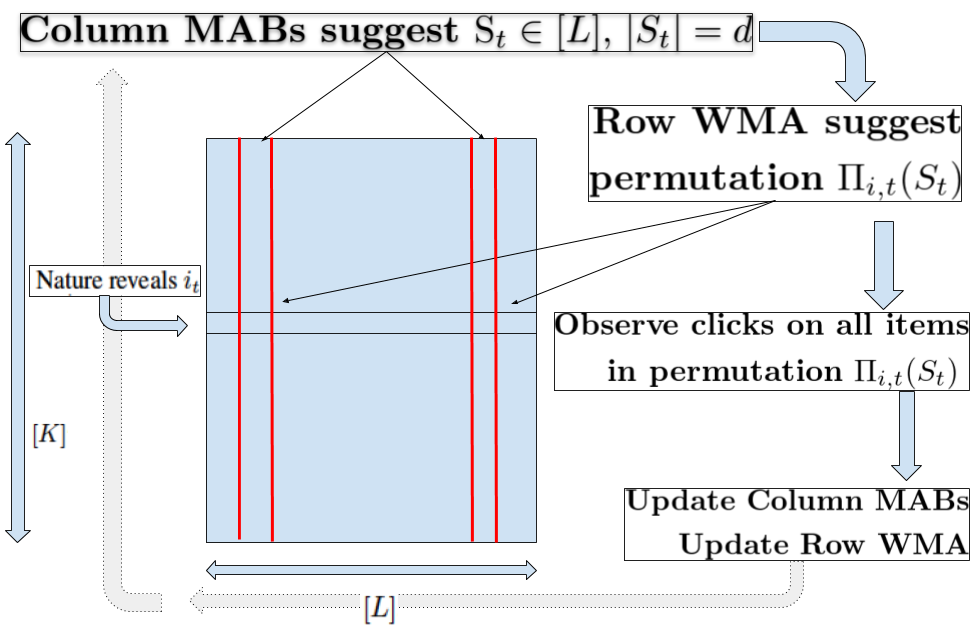
\includegraphics[scale=0.2]{img/RankedBand.png}
    \caption{Latent Ranked Bandit in rank $d=2$ scenario.}
    \label{fig:rankedbandit}
    \vspace*{-1em}
\end{figure}

Since the user feedback is observed on every column in $J_t$, we can compute the reward for all $d!$ permutations of $J_t$. This can be then used to update WMA$_{i_t,J_t}(n)$.    An illustrative diagram of the entire process is shown in Figure \ref{fig:rankedbandit}.

%Since, we observe all the clicks by user $i_t$ (total information),


\begin{algorithm}
\caption{Latent Ranker Algorithm}
\label{alg:latent-rank}
  \begin{algorithmic}[1]
  \State \textbf{Input:} Rank $d$, horizon $n$.
  \State Initialize MAB$_k(n)$ for $i=1,...,d$
  \State Initialize WMA$_{i,J}(n)$ for $i \in [K], J \subset [L], |J| = d.$
    \For{$t = 1, \dots, n$}
      \State User $i_t$ comes to the system
      \For{$k = 1, \dots, d$}
      %\State // Choose $d$ items from $d$ column MABs
      \State $\hat{{\ell}}_{k,t} \leftarrow$ suggest item $MAB_k(n)$
      \If{$\hat{{\ell}}_{k,t} \in \{ \ell_{1, t},\dots,\ell_{k-1, t}\}$}
      \State ${\ell}_{k,t} \leftarrow$ select arbitrarirly from the remaining
      \Else
      \State $\ell_{k,t} \leftarrow \hat{\ell}_{k,t}$
      \EndIf
      \EndFor
      \State $(\tilde{\ell}_{1,t},\tilde{\ell}_{2,t},\dots,\tilde{\ell}_{d,t} )\leftarrow$ WMA$_{i_t,\{ l_{1,t},...,l_{d,t} \} }$ %by sampling  according to $p_{i_t,1},p_{i_t,2},\dots,p_{i_t,d!}$.
      %by sorting descendingly according to $w_{i_t,1},w_{i_t,2},\dots,w_{i_t,d}$.
      \State Let  $\{ r_{t}(\ell_{1,t}), r_{t}(\ell_{2,t}),\dots,r_{t}(\ell_{d,t}) \}$ be the user feedback.
      \State Let $f_t(\ell_{i,t}) = \max \{ r_t(\ell_{1,t}),...,r_t(\ell_{i-1,t}),r_t({\ell}_{i,t}) \} - \max \{ r_t(\ell_{1,t}),...,r_t(\ell_{i-1,t}) \}$ 
      \State update(MAB$_{k}(n)$, reward = $f_t(\ell_{k,t})$, arm = $\hat{\ell}_{k,t}$)
      \State update(WMA$_{i_t,J_t}$,$\{ r_t(\ell_{1,t}),...,r_t(\ell_{d,t})\}$ )
    \EndFor
%    \Procedure{UpdateColumnMAB}{}
%    \For{$k = 1, \dots, d$}
%    \State Update MAB$_k(n)$ with feedback $f_{k,t} = \max_{j\in [k]} r_t(i_t, \ell_{j,t}) - \max_{j\in [k-1]} r_t(i_t,\ell_{j,t})$
%    % where $J_t[1: k] = \lbrace r_{t}({\ell}_{1,t}), r_{t}({\ell}_{2,t}),\dots,r_{t}({\ell}_{k,t})\rbrace$
%    \EndFor
%\EndProcedure
%\Procedure{UpdateRowWMA}{$i_t$}
%	\For{$k=1,2,\dots,d!$}
%	\State $r_k = 0$ \Comment{Calculate weighted sum of rewards}
%    \For{$j = 1, \dots, d$}
%    \State $r_{k} = r_{k} + \frac{1}{j}r_{t}(\tilde{\ell}_{j,t})$
%    \EndFor
%    \State $w_{i_t,k} = w_{i_t,k} + r_k$  \Comment{Update weights}
%    \EndFor
%	\For{$k = 1, \dots, d!$}
%	\State $p_{i_t,k} = \dfrac{\exp(w_{i_t,k})}{\sum_{b=1}^{d!} \exp(w_{i_t,b})} $ %\Comment{Update probabilities}
%	\EndFor
%\EndProcedure
  \end{algorithmic}
\end{algorithm}

\todoan{Probably need to add a bit more explanation about the rewards of MABs}